\section{Data Description}

\subsection{The tool}
The EPA ECOTOX database contains almost 1,000,000 ecotoxicological test results from almost 12,000 chemicals and about 13,000 taxa \citep{usepa_ecotox_2019} and represents the largest publicly available collection of ecotoxicological test data. However, it constitutes only a collection of test results without aiming for summarising the information, which leads to the problem of multiple test results occurrences for individual chemicals. To tackle this Standartox introduces filter and aggregation methods that enable the derivation of single ecotoxicological endpoints for specific test parameter combinations. Hence, Standartox contains about 600,000 ecotoxicological test results comprising roughly 8000 distinct chemicals and taxa. The data can be restricted to three endpoints (XX50, LOEX and NOEX) and filtered to 23 distinct effect groups (e.g. mortality, population, growth). Furthermore, the data can be refined to five chemical classes (e.g. pesticides, metals, drugs) as well as to species-specific habitats (e.g. freshwater, marine, terrestrial) and regions (e.g. Europe, South America).


Different parameters in order to filter the test data, such as compound-specific parameters, including the CAS number, the concentration type (e.g. Active Ingredient, Formulation) or the chemical class (e.g. insecticides, metals) as well as taxon-specific parameters, including common taxonomic groups (e.g. Daphniidae, algae), the habitat (e.g. freshwater) or the regional occurrence (e.g. Europe, Asia) of the organisms can be chosen. Furthermore, users can refine the results to specific test durations (in hours), effect groups (e.g. mortality, population, growth) and endpoints (EC\textsubscript{50}, LOEC or NOEC). As the method of aggregation users can choose the minimum, the maximum, or the geometric mean.



%%%%%%%%%%%%%%%%%%%%%%%%%%%% CONTINUE HERE %%%%%%%%%%%%%%%%%%%%%%%%%%%%%%%%%%%%%%






Standartox is a tool that allows to filter and aggregate ecotoxicological test results to derive single exposure endpoints for individual chemicals. It can either be accessed through the APP (Figure \ref{fig:app}) or the API \ref{tab:api-endpoints} together with the R-package standartox (Code example \ref{listing:standartox-example}). 




%% TODO Add units part here







\pagebreak

\begin{table}[ht]
  \caption{Input parameters for the Standartox Web application and the R-package standartox.}
  \label{tab:app-parameters}
  \centering
\begin{tabular}{ll}
  \hline
  parameter & example \\ 
  \hline
  cas & 7758987, 2921882, 1912249 \\
  concentration\_type & active ingredient, formulation, total \\
  chemical\_class & fungicide, herbicide, insecticide \\
  taxa & Oncorhynchus mykiss, Rattus norvegicus, Daphnia magna \\
  habitat & marine, brackish, freshwater \\
  region & africa, america_north, america_south \\
  duration & 24, 96 \\
  effect & Mortality, Population, Growth \\
  endpoint & NOEX, XX50, LOEX \\
  vers & 20190912 \\
  \hline
\end{tabular}
\end{table}


\pagebreak

\begin{table}[ht]
  \caption{Application programming interface (API) endpoints, Http methods, Requests and Response objects. Object is abbreviated with obj.}
  \label{tab:api-endpoints}
  \centering
\begin{tabular}{cccc}
  \hline
  Endpoint & Http Method & Request & Response \\ 
  \hline
  /catalog & POST & \makecell{Standartox \\ version string} & \makecell{Catalog object of \\ possible filter parameters \\ JSON obj.}    \\[0.5cm]
  /filter & POST & \makecell{Standartox filter \\ parameters (Table \ref{tab:app-parameters})} & \makecell{Filtered Standartox data \\ serialized R data.frame \\ R fst:: \citep{klik_fst_2019} obj.}   \\[0.5cm]
  /aggregate & GET & / & \makecell{Aggregate function \\ serialized R function \\ R .rds \citep{rcoreteam_language_2017} obj.}    \\[0.5cm]
  /meta & POST & \makecell{Standartox \\ version string} & \makecell{Meta data on request \\ JSON obj.}    \\
  \hline
\end{tabular}
\end{table}

\pagebreak

Standartox is designed to foster chemical risk assessment (CRA). Due to an increased amount of available ecotoxicological test data, it becomes fundamental to provide and distribute such information in adequate formats, both easily accessible for humans and easily processable for machines. 






In order to locate ecotoxicological test data, researchers can rely on individual test results reported in publications, on compiled and published data sets \citep{malaj_organic_2014, morrissey_neonicotinoid_2015} or on data bases such as the Pesticide Property Data Base (PPDB) \citep{lewis_international_2016}. Each approach has its limitations though. Collecting toxicity information from individual publications is laborious and using already compiled data from publications or published data bases is often limited to specific groups of chemicals, such as pesticides, biocides etc. Additionally it is not always clear whether presented effect values are aggregated or single specific tests have been selected. These resources can provide out of date data and rarely provide sophisticated means to directly process the data.



Standartox overcomes these paucities by making use of the quarterly updated EPA ECOTOX data base, the largest publicly available collection of ecotoxicological test information. In doing so, Standartox allows for a quick access to ecotoxicological test data, not being confined to specific chemical classes. Furthermore, Standartox constitutes not only a one-time compiled data set but rather a scalable method that can steadily incorporate new ecotoxicological test data in an automated manner, allowing for constant improvement of toxicity estimations over time. Data retrieval is streamlined and can be easily done via the APP or the R package. On top of filtering the data, Standartox provides means to aggregate results from multiple ecotoxicological tests to retrieve single exposure endpoints for specific chemical, taxon and test parameter combinations. Test results for each chemical in the filtered data set are thereby aggregated by calculating the minimum, the geometric mean or the maximum. Standartox returns then a filtered and an aggregated data set. Besides, Standartox allows users to access older versions of the data base as well and is created as open source software and therefore a fully reproducible method.




\subsection{Accuracy Assessment}
Other initiatives harmonizing the large number of ecotoxicological test results were also developed recently. They partly aim for overlapping goals, yet have limitations or objectives that differentiate them from Standartox. Since 2006, the PPDB provides validated ecotoxicological information on pesticides \citep{lewis_international_2016}. In order to asses the validity of the Standartox aggregation approach, we compared Standartox results with effect values from the PPDB (n=3601) for the same chemicals (Figure \ref{fig:standartox_ppdb_diff}). This showed that 91.3\% of the Standartox values diverge by less than a factor of ten from the PPDB values. Considering only Standartox values for which at least five or ten tests were aggregated the value increases to 91.7\% and 93.4\%, respectively. Admittedly a few Standartox values diverge by a large margin.

\begin{figure}
    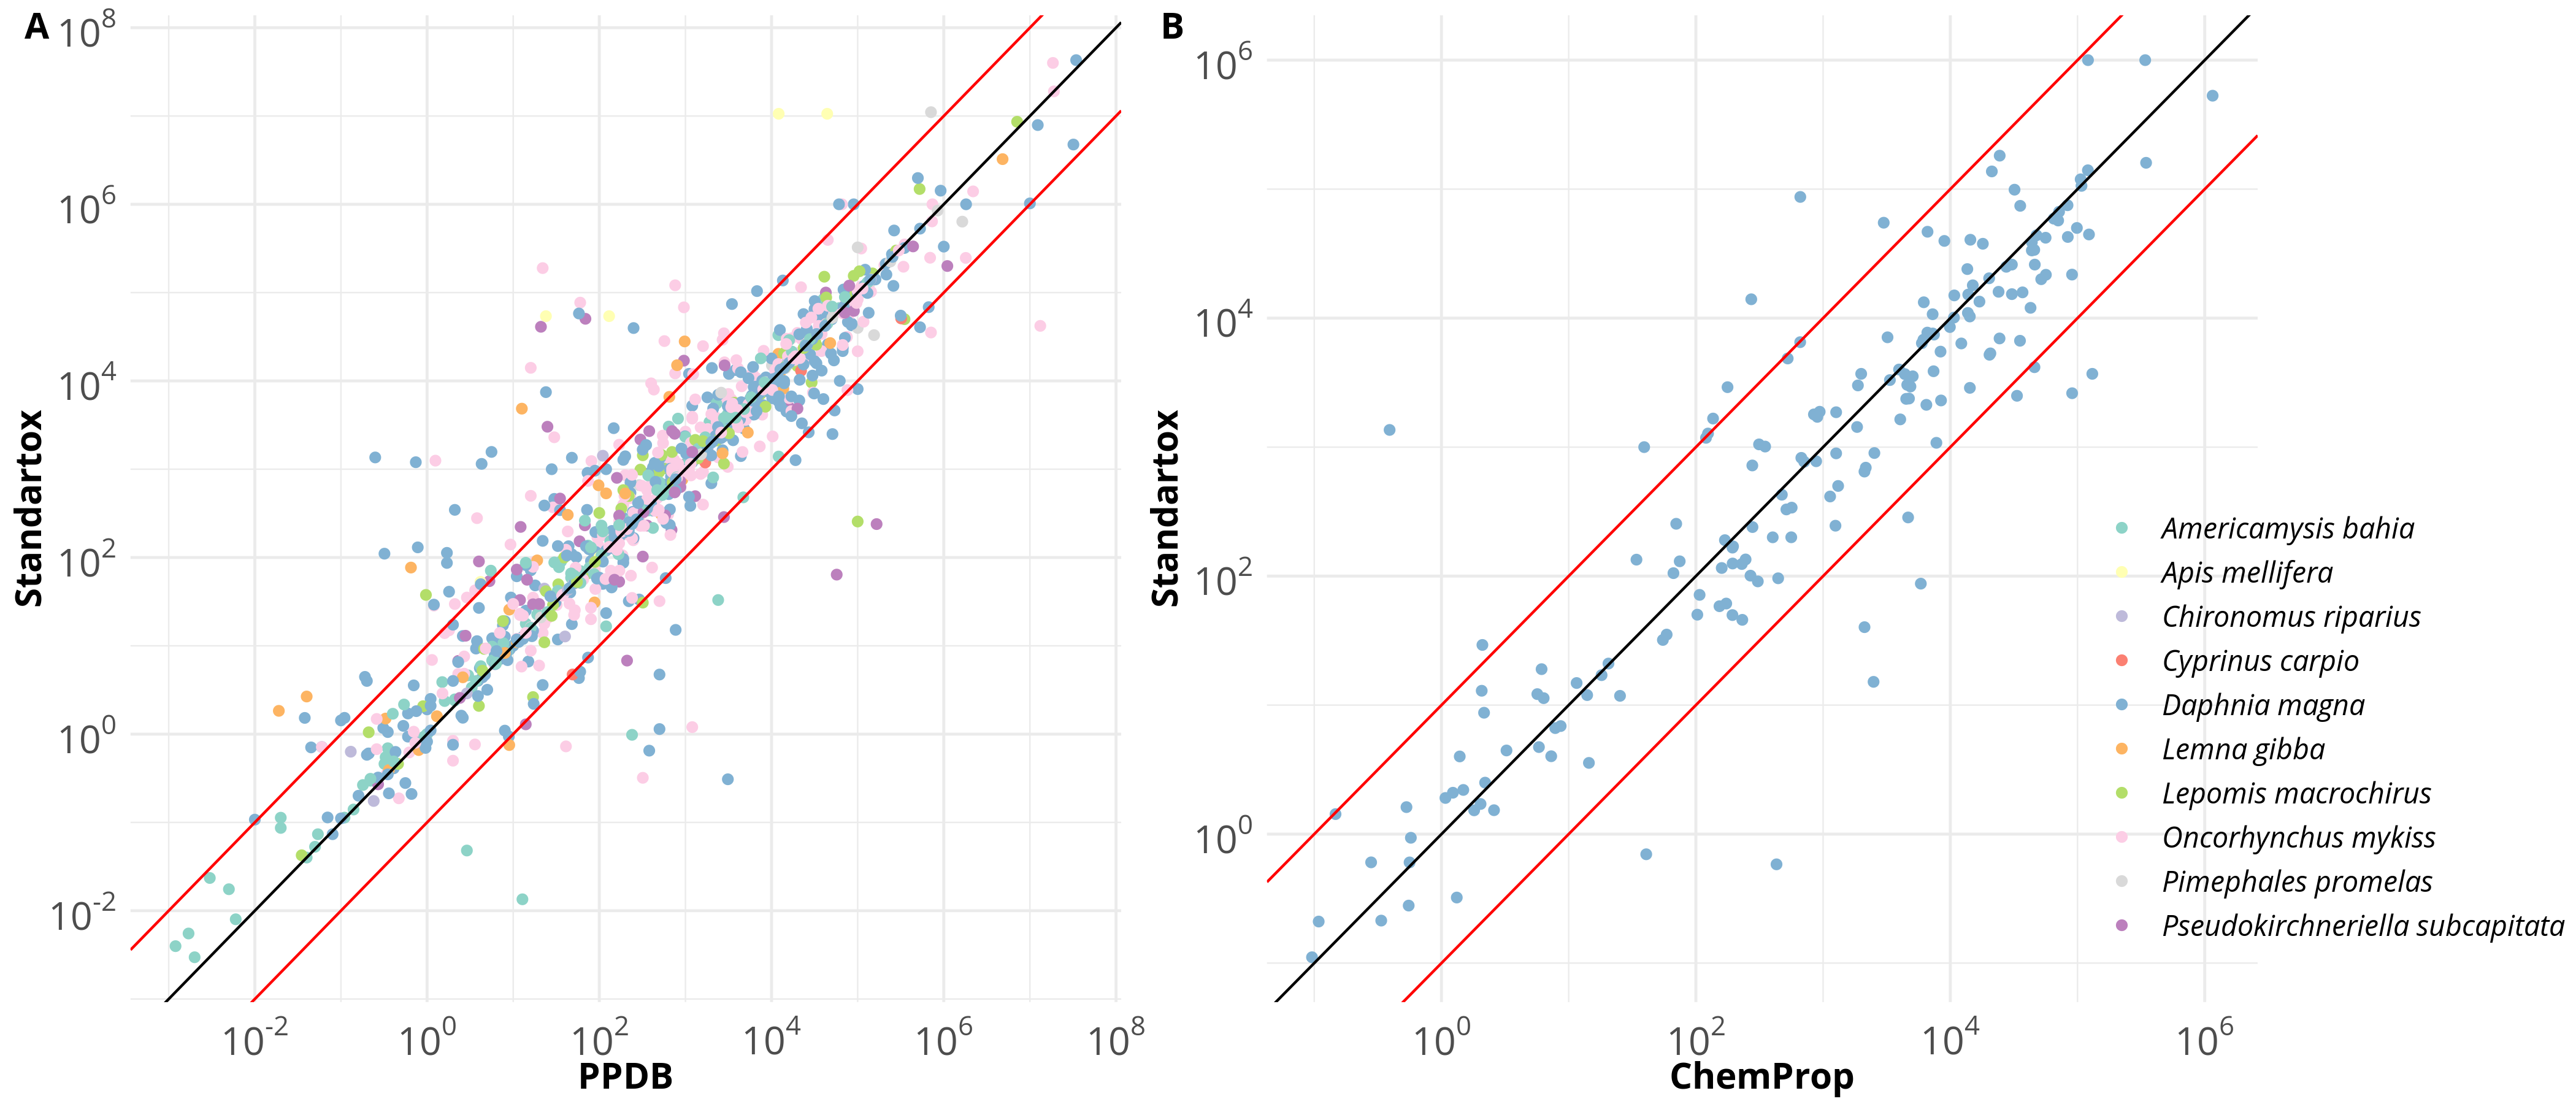
\includegraphics[width=1\linewidth]{article/figures/gg_ppdb_stan_compare_continous.png}
    \caption{Comparison between Standartox and PPDB values. The black line marks exact coherence and red lines mark a divergence of a factor of 10. Compared organism groups are color coded.}
    \label{fig:standartox_ppdb_diff}
\end{figure}

The Network of reference laboratories, research centres and related organisations for monitoring of emerging environmental substances (NORMAN) focuses on assembling river basin specific pollutants from studies and databases \citep{von_der_ohe_new_2011}. The EnviroTox data base \href{https://envirotoxdatabase.org/} which also uses, amongst others the EPA ECOTOX data base as an input was recently published \citep{healthandenvironmentalsciencesinstitutehesi_envirotox_2019, connors_creation_2019}. In comparison to Standartox, EnviroTox focuses only on aquatic organisms and uses an qualitative algorithm to exclude unreliable test results, such as pre-filtering, for example the data to fish, amphibian invertebrate and algae taxa, to test durations of above 24 hours and aquatic taxa only. Besides, they add additional information on toxicity endpoints, such as acute or chronic classifications and mode of action assignments. In contrast, Standartox doesn't refine to specific test durations, but leaves it up to the user to decide on such parameters. The EnvirTox data base also allows for an aggregation of test results to derive single toxicity values for individual taxa whereas Standartox performs this aggregation for individual chemicals. Comptox, is a web tool published by the EPA which, similar to Standartox allows for filtering test results, the retrieval of additional chemical information and predicting toxicity properties, such as 48 h \textit{Daphnia magna} LC\textsubscript{50} values. However, toxicity predictions are limited to some standard organisms (e.g. \textit{Daphnia magna}), and the tool lacks the possibility to retrieve predicted values in an automated way \citep{williams_comptox_2017}. Petschick et al. (in submission) modeled risk threshold level equivalents for aquatic organisms by using ecotoxicological effect data from the EPA ECOTOX data base to support regulation. In summary, none of the above mentioned approaches aim for a holistic standardized aggregation method of exposure endpoints for individual chemicals and also lack the possibility for automated and scriptable user requests from common high level programming languages, such as R or Python. Along with newly created ecotoxicological data bases here, methods of how to efficiently store ecotoxicological data are also proposed as can be seen in the MAGIC Knowledge Base \citep{bub_graphing_2019}. This recent increase of efforts to compile ecotoxicological test data bases clearly emphasizes the need for holistic and automated analyses of large-scale ecotoxicological data. 

\subsection{Limitations}
Since the data in Standartox merely represents a sample of the actual toxicity of chemicals on organisms, it has to be stated that the returned Standartox values are subject to change. New studies will be published and constantly incorporated into EPA ECOTOX data base and therefore into Standartox, improving the toxicity estimates. However, we expect values of well tested chemical-organism combinations to be relatively stable. A future analysis on the smallest number of tests needed to return trustworthy results, could shed more light on this aspect. Furthermore, toxicity test results are certainly influenced by individual tests parameters, such as pH, temperature or conductivity amongst others \citep{rosenkrantz_influence_2013, li_temperature_2011}. Such information is not included in the aggregation performed by Standartox, since the EPA ECOTOX data base only provides sparse records on those. Most frequently provided test parameters (and their percentage) are medium temperature (77\%), pH:56\%, hardness:27\%, dissolved oxygen:18\%, Alkalinity:15\% and salinity:9\%. Others are provided for less than 5\% of the tests. A text-mining approach, iterating through the individual publications could potentially increase this number. However, we argue that using the geometric mean as an aggregate allows for an adequate estimation of the toxicity of a chemical towards an organism group. We chose the geometric mean in comparison to the arithmetic mean, since it is considerably less influenced by outliers and is suitable for skewed data. Also, the geometric mean is preferable over the median, since the median completely ignores the influence of large or small values, making it unreliable for small data sets <CITATION GEOMETRIC MEAN>.


%%%%%%%%%%%%%%%%%%%%%%%%%%%%%%%%%%%%%%%%%% TODO %%%%%%%%%%%%%%%%%%%%%%%%%%%%%%%%%%%%%%%%%%
\iffalse
- rename subsections as such:
    
\subsection*{Accuracy Assessment}


\subsection*{Perspective}

- can also be incorporated in EPA Dashboard
- Identify also underrepresented regions concerning organisms.
1) \citep{staveley_challenge_2016} describe what is necessary for future ecotoxicology.
2) Compare Standartox with predictions here: https://comptox.epa.gov/dashboard/predictions/index
- \citep{gadaleta_new_2018} what does this software exactly do an how to access it?
\fi
%%%%%%%%%%%%%%%%%%%%%%%%%%%%%%%%%%%%%%%%%% OLD %%%%%%%%%%%%%%%%%%%%%%%%%%%%%%%%%%%%%%%%%%%

\iffalse
SSD try to extrapolate effects of chemicals towards organisms from species to a community level by fitting a statistical distribution to toxicity test results on organisms of different trophic levels in order to derive concentrations at which a specific fraction of organisms are effected (often at 5\% - HC\textsubscript{5} \citep{posthuma_species_2002}. Figure \ref{fig:ssd-isoproturon} shows an example of a SSD and the derived HC\textsubscript{5} value (red dassed line) created for the herbicide Isoproturon. TUs are another indicator of effects of chemicals on organisms. They are calculated by dividing a measured concentration (c) by an EC\textsubscript{50} value (cf. Equation \ref{eq:tu}).

\begin{equation}
    TU_i = \frac{c_i}{\ecfifty}
    \label{eq:tu}
\end{equation}

\begin{figure}[h!]
    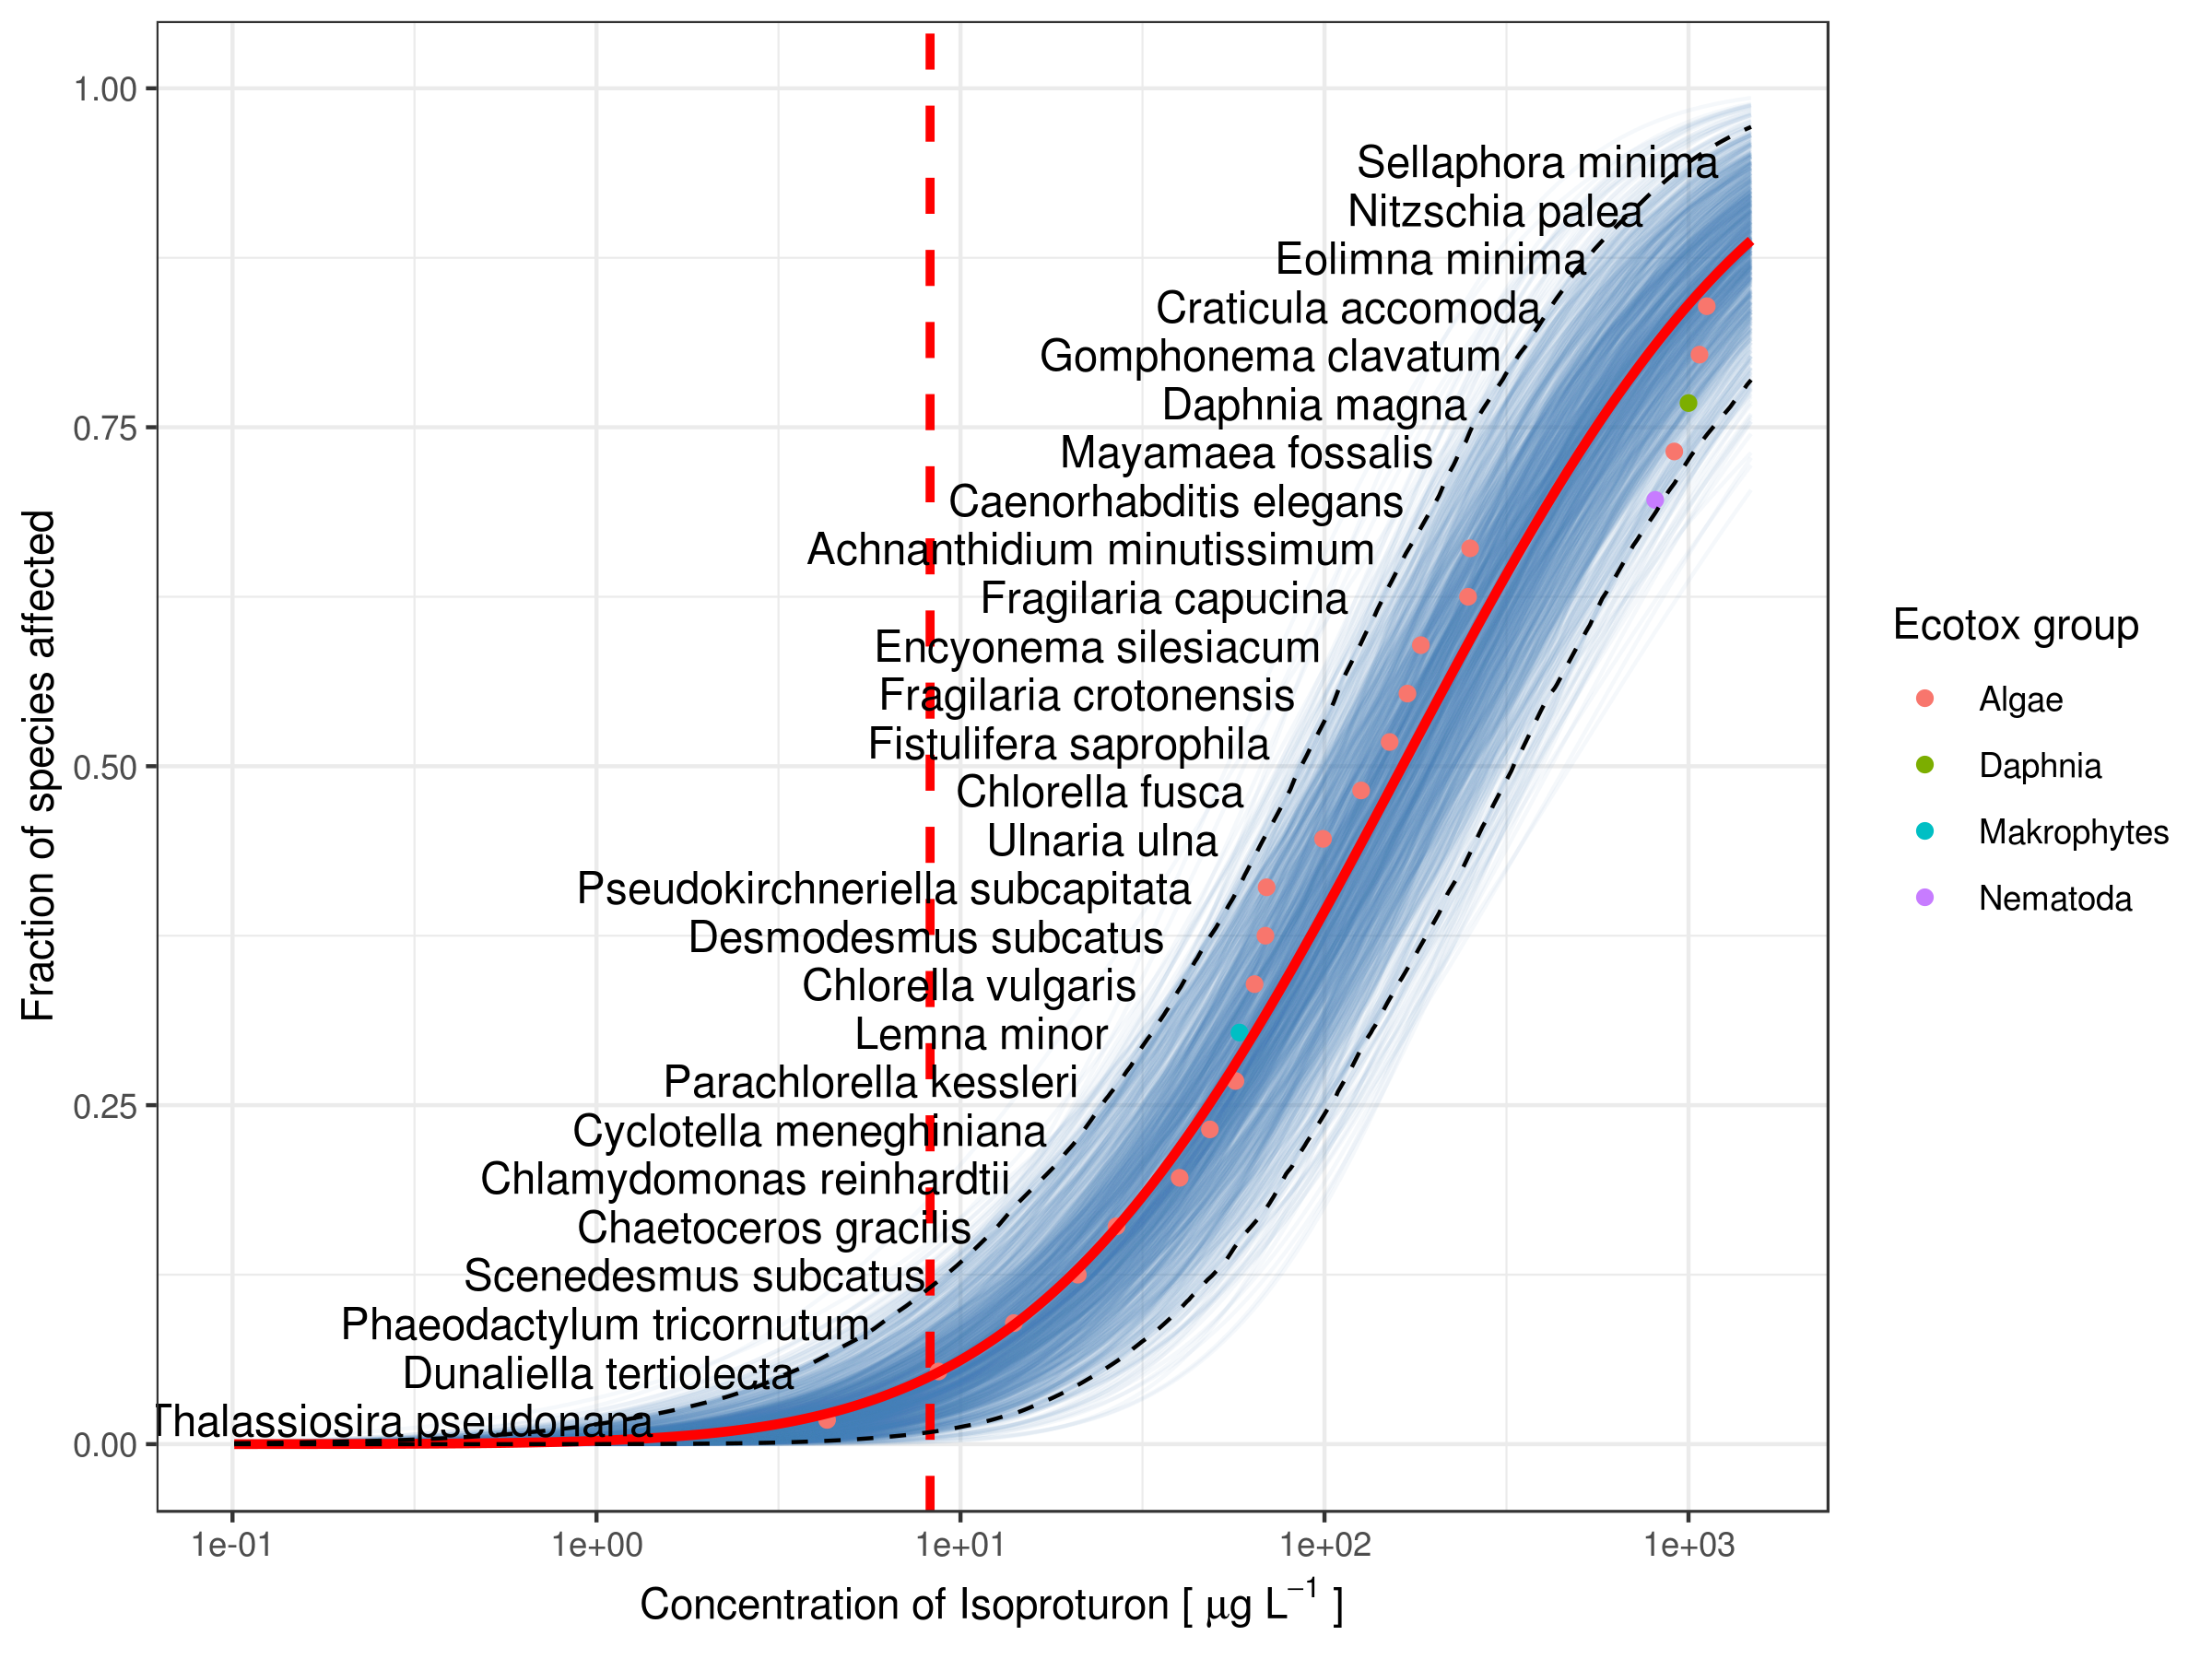
\includegraphics[width=1\linewidth]{article/figures/ssd2_boot.png}
    \caption{SSD plot showing the susceptibility of organisms towards the herbicide Isoproturon. The red line represents the fit and the red dashed line marks the HC\textsubscript{5} value, which is a common measure in CRA. The legend denotes common organism groups used in ecotoxicology.}
    \label{fig:ssd-isoproturon}
\end{figure}

Besides that, two cleaning steps can also be chosen. Firstly the application allows to exclude test results exhibiting concentrations that are higher than the actual water solubility of the respective chemical at \ang{20} C. Secondly the user can choose to exclude outliers (cf. Table \ref{tab:scripts-app}). The outliers are selected as values that exceed lower (0.25) and the upper (0.75) quartile by 1.5 times the inter-quartile range.

\subsection*{Identify chemicals to be tested}
There is a clear need in ecotoxicology for harmonised approaches to collect ecotoxicological data as other data base compilation attempts recently published show. Hitchock et al. \citet{hitchcock_improving_2018} argue for an increased awareness concerning newly published ecotoxicological test results to facilitate meta analyses across studies. Important statistical parameters, such as mean estimates, variances and sample sizes. Likewise, state variables, including medium temperature, pH, mineral contents or organism age and sex should be reported (if not in the text, in an online repository). Standartox doesn't include such information mainly because the EPA ECOTOX reports only a few of these variables. A future research aim could be to use machine learning techniques to retrieve this information from the referenced articles.
Above all, recent studies showed that, in defiance of many regulation efforts \citep{schafer_future_2019} chemicals can still cause strong adverse effects on organisms and in turn on the environment. Neonicotinoids, a group of insecticides was for example related to declines in insectivorous birds \citep{hallmann_declines_2014} and fish yields due to cascading food web effects \citep{yamamuro_neonicotinoids_2019}. Standartox provides means to synthesise ecotoxicological test data, thereby identify research gaps. 

\begin{figure}
    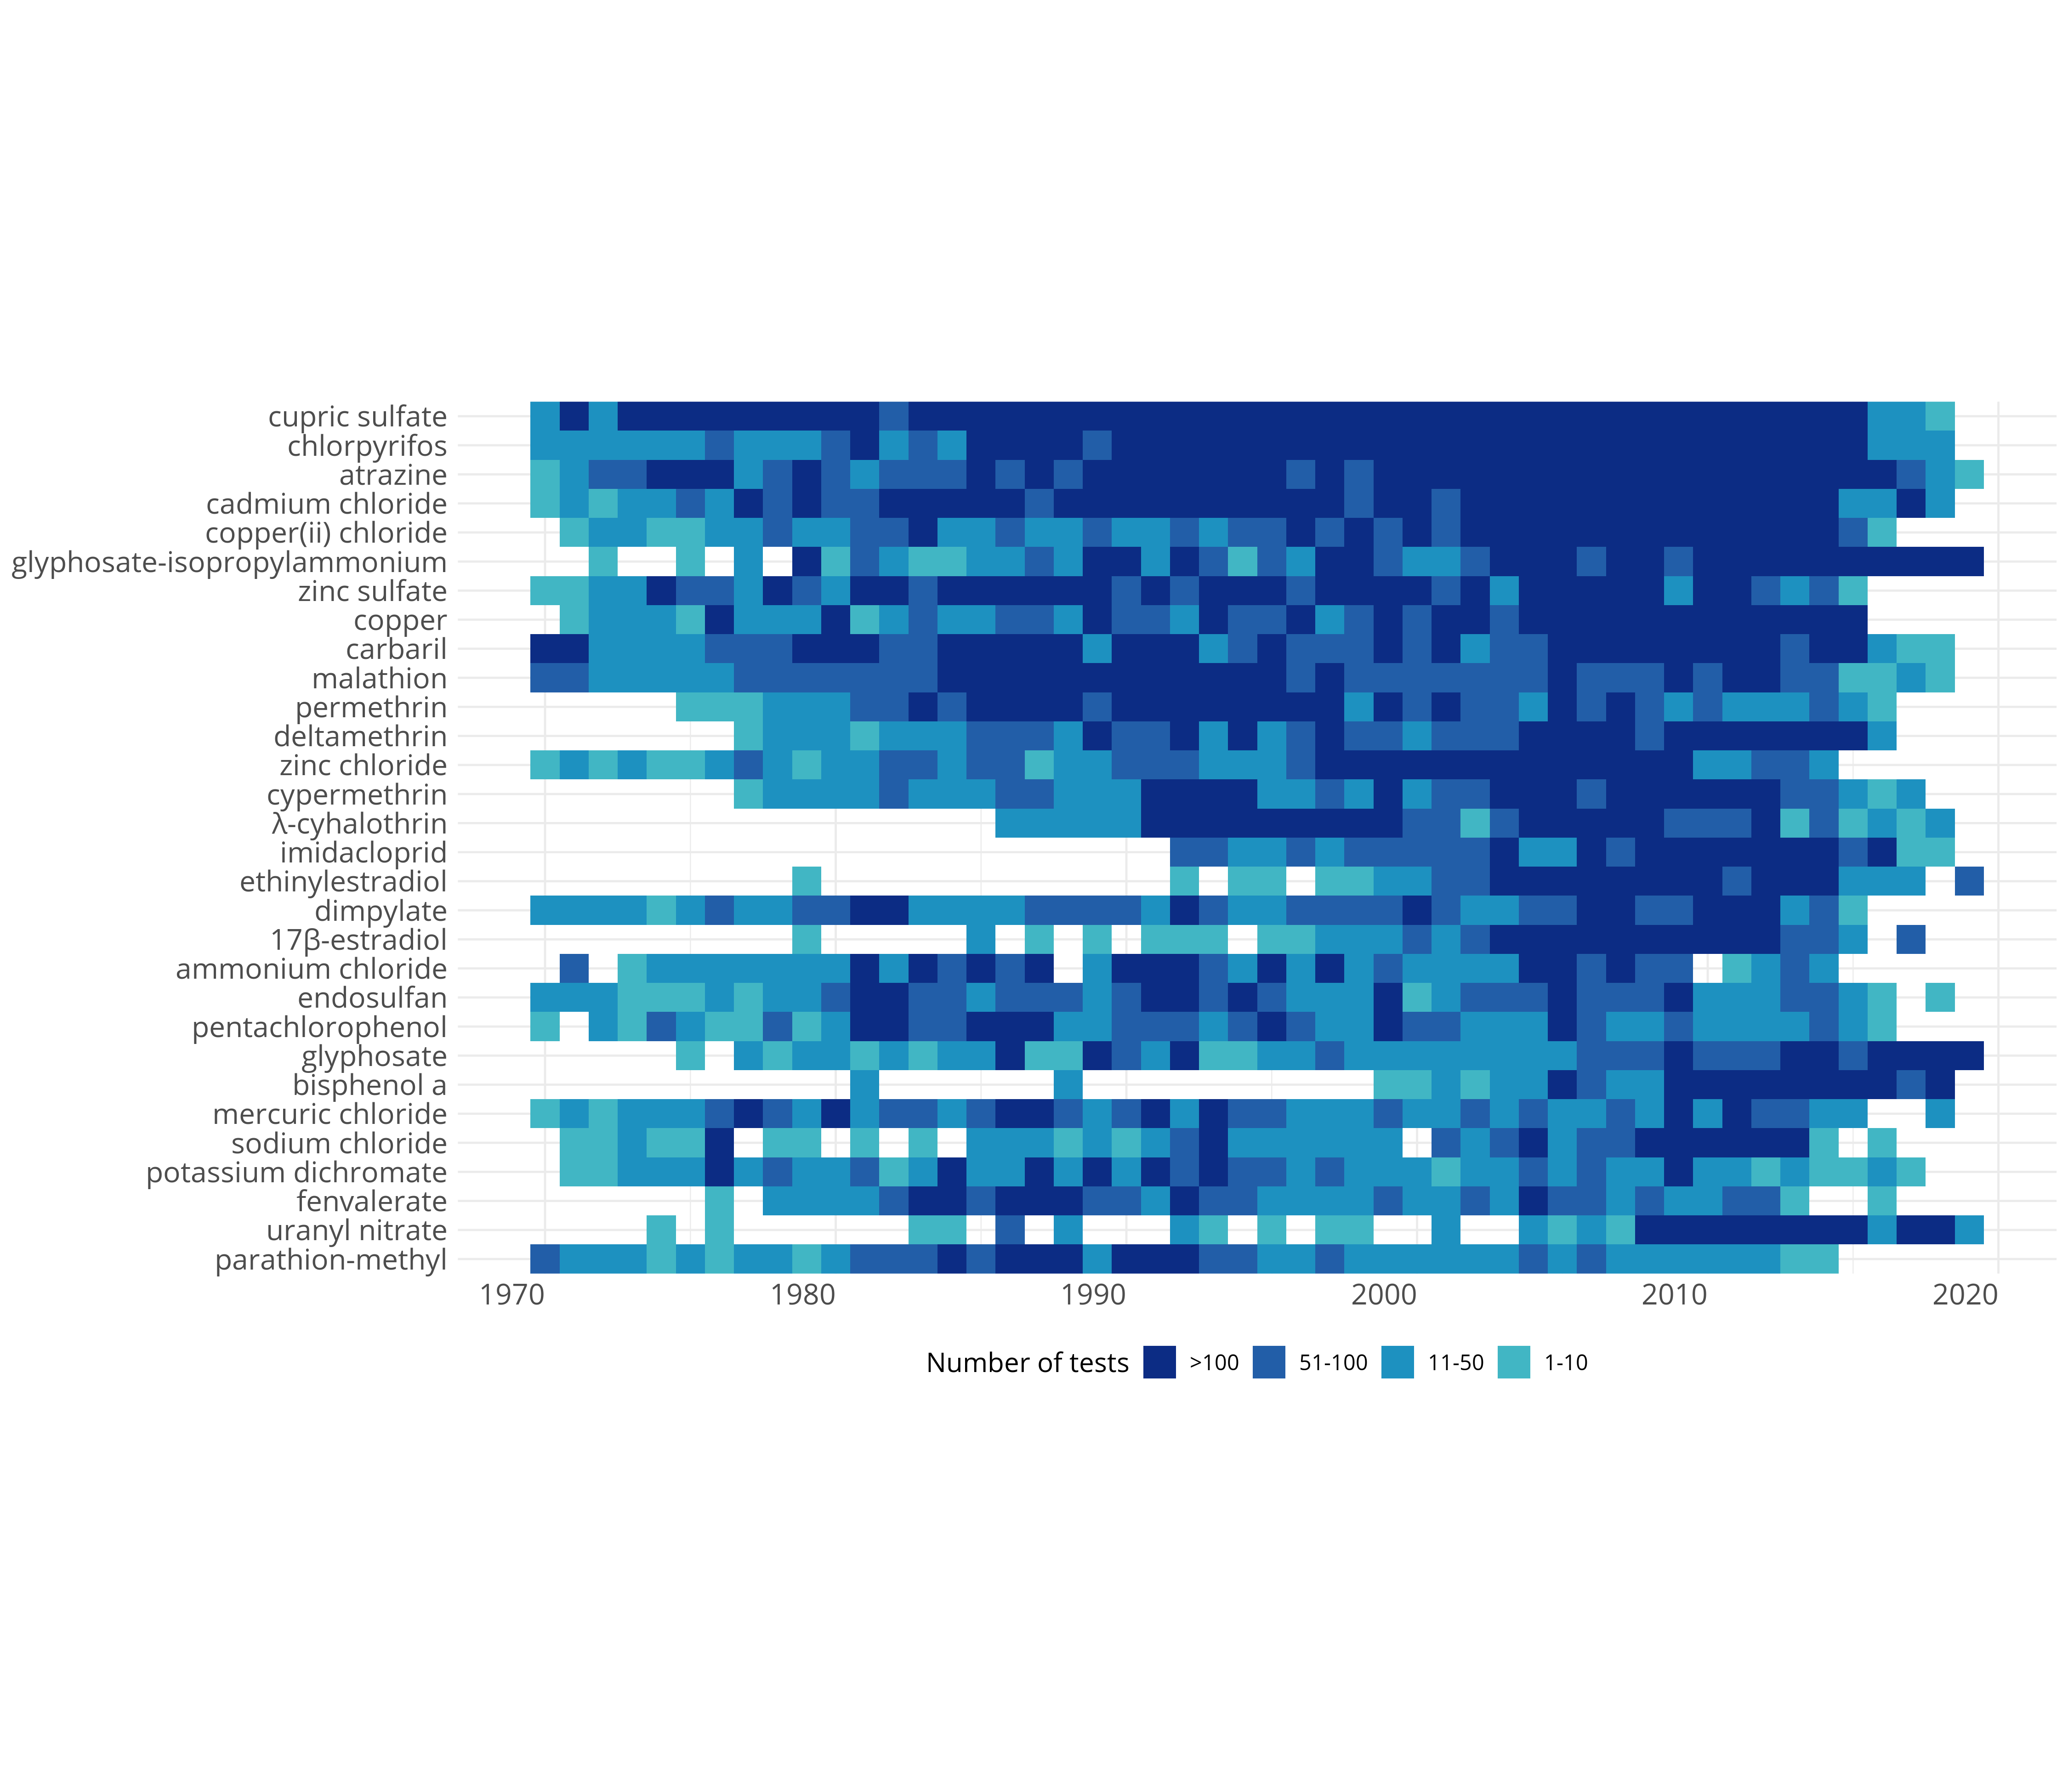
\includegraphics[width=1\linewidth]{article/figures/heatmap_tests_n.png}
    \caption{30 most tested chemicals in EPA ECOTOX.}
    \label{fig:standartox_ppdb_diff}
\end{figure}



\fi